
\chapter{Basic Concepts about Computing Performance\label{chpt:computing-performance}}

In addition to the theory work, the performance of the code being
developed is also an important aspect of this thesis. It is essential
to have a fast and accurate method. To evaluate code in a strict and
systematic way, some basic concepts of computing performance are listed
here. 

\section{Algorithm complexity}

Algorithm complexity is a crucial criteria for sequential code. A
definition is given below.

Let $f$ and $g$ be two real (or even complex) functions defined
over the natural numbers $\mathbb{N}$. We write
\begin{equation}
f=O(g)
\end{equation}
if there is a constant $c>0$ such that from certain number $n>n_{0}$
we always have $\left|f(n)\right|\leq c\left|g(n)\right|.$ The $O$
is also named as the big-O notation \citep{Complexity}, or order
of growth. Figure \ref{fig:order-of-growth} shows the growth tendency
of some frequent functions; from this we can conclude the following:
\begin{equation}
O(1)>O(\log_{2}n)>O(n)>O(n\log_{2}n)>O(n^{2})>O(2^{n})>O(n!)
\end{equation}

\begin{figure}[h]
\begin{centering}
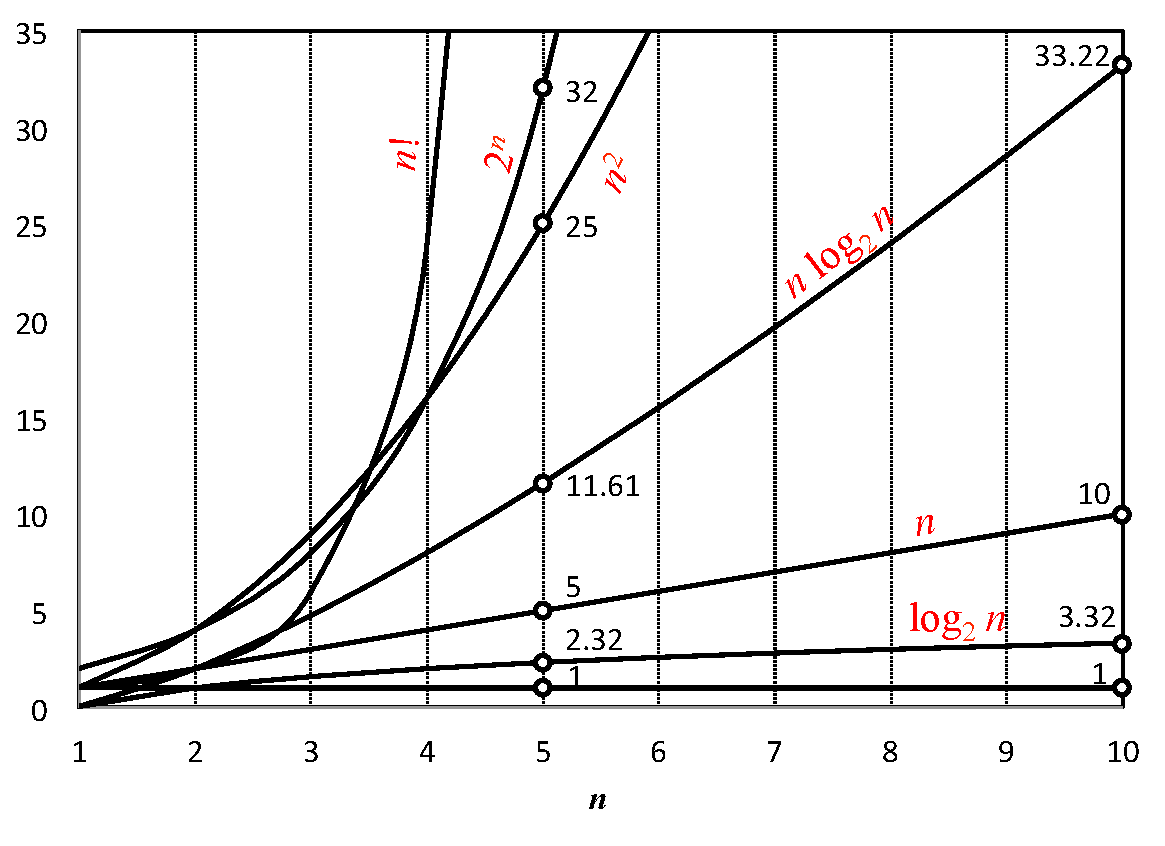
\includegraphics[width=0.65\textwidth]{_figure/orders-of-growth}
\par\end{centering}
\caption{Function growth\label{fig:order-of-growth}}
\end{figure}

In this thesis, the big-O notation is used to measure algorithm complexity.
Other notations can also be used for the same purpose, such as:
\begin{itemize}
\item $f=o(g)$ if $f(n)/g(n)\rightarrow0$, $n\rightarrow\infty$
\item The inverse of big-O notation $f=\Omega(g)$ if $g=O(f)$
\item The notation $f=\Theta(g)$ means that both $f=O(g)$ and $g=O(f)$
hold, and we can also say they are of the same order.
\end{itemize}
In a code we always search algorithms with a lower algorithm complexity.
Ideally, the implementation of code matches the model and have the
same growth tendency as its complexity, but in the practical case,
overheads and memory delay can also limit the performance. \textcolor{red}{(part
to be modified to adapt implementation results)}

\section{Roofline model and memory delay}

The simplest model aiming to distinguish whether a piece of code is
limited by the computing power (CPU) or the memory bandwidth (RAM
to Caches) is the roofline model \citep{Williams_2009_roofline} for
single loop:
\begin{equation}
P=\min\left(P_{\max},\,I\cdot b_{\mathrm{S}}\right)\label{eq:roofline}
\end{equation}
where

\begin{tabular}{l>{\raggedright}p{0.9\textwidth}}
$P$ & is the applicable peak performance of a loop, assuming that data comes
from the level 1 cache, of unity $\mathrm{GFlop/s}$. \tabularnewline
$I$ & is the computational intensity (“work” per byte transferred) over
the slowest data path utilized, of unity $\mathrm{Flop/Byte}$. \tabularnewline
$b_{\mathrm{S}}$ & is the applicable peak bandwidth of the slowest data path utilized,
of unity $\mathrm{GByte/s}$.\tabularnewline
 & \tabularnewline
\end{tabular}

As shown in figure \ref{fig:The-roofline-model}, the overall performance
is limited by both the peak performance and the memory bandwidth.
The computational intensity $I$ depends on the code, while the other
two terms in eq. (\ref{eq:roofline}) depend on hardware. The optimal
use of resources occurs at the intersection point.

\begin{figure}[h]
\begin{centering}
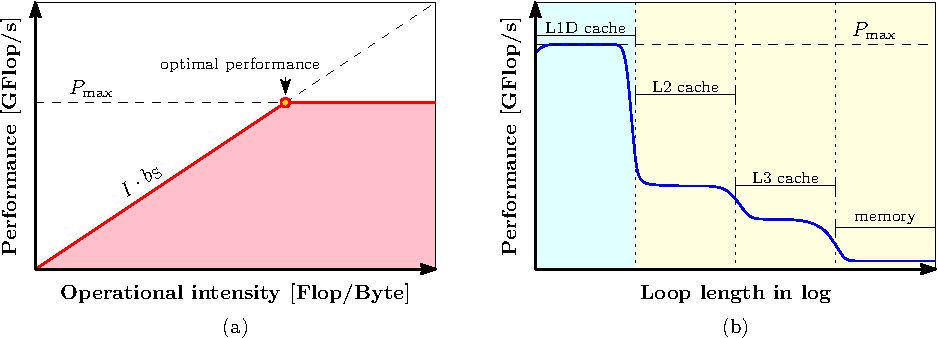
\includegraphics[width=1\columnwidth]{_figure/roofline}
\par\end{centering}
\caption[The roofline model and performance pattern]{The roofline model and performance pattern. (a) The roofline model.
(b) Performance pattern of a simple loop with respect to the loop
length in logarithm. The blue part is limited by operation execution,
and the yellow part is limited by memory bottleneck. \label{fig:The-roofline-model}}
\end{figure}

The roofline model can give an idea of whether the diminuition of
algorithm complexity is the most important optimization strategy,
because it only counts the number of operations. In most cases, avoiding
slow data paths is the key to performance optimization.

As shown in figure \ref{fig:Memory}, the memory hardware has hierarchical
architectures. The fastest ones are the registers included in the
microprocessor, which are used for temporary storage of data, instructions
and addresses required by the arithmetic logic unit (ALU) and the
control unit (CU) in CPU during execution of a program. The lowest
is normally the input/output (I/O) process. The reading strategy of
data (contiguous or not), as well as the size and initialized location
of arrays, both play pivotal roles in the overall computing performance.

\begin{figure}[h]
\begin{centering}
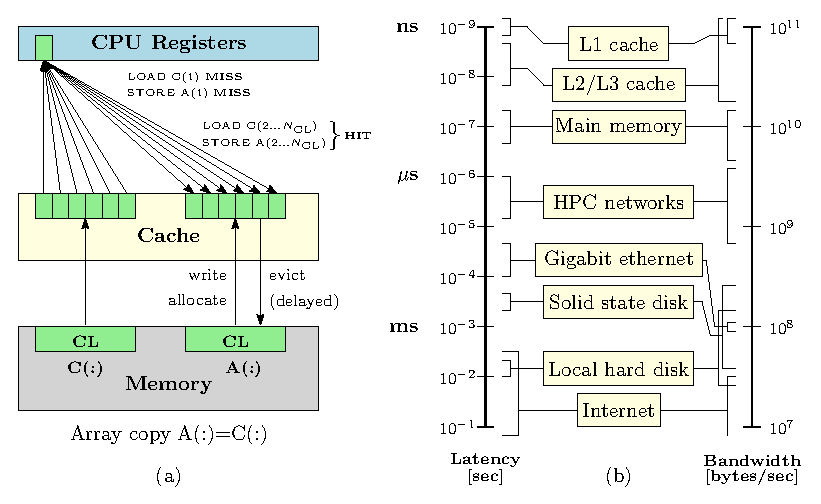
\includegraphics{_figure/memory}
\par\end{centering}
\caption[Memory usage in hardware level]{Memory usage in hardware level \citep{LRZ-cours}. (a) An example
of array copy A(:)=C(:). Caches are organized in cache lines (CL),
only complete cache lines are transferred between memory hierarchy
levels (except registers). HIT/MISS: Load or store instruction does/doesn't
find the data in a cache level. (b) Computing latency and memory bandwidth
vary by magnitude, from the fastest cache transfers to the lowest
processes.\label{fig:Memory}}
\end{figure}


\section{Scalability of parallelized code}

For parallelized code, scalability is the key issue. Highly scalable
codes can take advantage of numerous nodes of HPC centers, so that
single core performance no longer matters. 

The speed-up is defined as:
\begin{equation}
S(N)=\dfrac{t(1)}{t(N)}
\end{equation}

And the relative efficiency
\begin{equation}
E(N)=\dfrac{S(N)}{N}=\dfrac{t(1)}{Nt(N)}
\end{equation}

$S(N)\sim N$ or $E(N)\sim100\%$ means the application scales. By
contrast, $S(N)<N/2$ or $E(N)<50\%$ means the application does not
scale. 

Amdahl's Law gives the theoretical speedup in latency of the execution
of a task at fixed workload:
\begin{equation}
S(N)=\dfrac{1}{\alpha_{\mathrm{s}}+\alpha_{\mathrm{p}}/N}
\end{equation}
where $\alpha_{\mathrm{s}}$ is the serial fraction and $\alpha_{\mathrm{p}}$
the parallel fraction of the source code. Therefore the overall computing
speed is limited by the unscalable part:
\begin{equation}
\lim_{N\rightarrow\infty}S(N)=\frac{1}{\alpha_{\mathrm{s}}}
\end{equation}
making it the focus we wish to reduce.

\section{Profiling and tracing toolkits}

There are several types of software and toolkits for performance evaluation.
They comprise two categories: profiling and tracing. A trace is a
collection of events or timestamps. A profile is a collection of timings.
Profiling tools are usually more simple and rapid, but for subroutines
that are called a large number of times, the overhead in time measurement
is not negligible. 

The tool used in this thesis is mainly VTune, where application execution
is interrupted every $\sim100\,\mathrm{\mu s}$ and information is
stored (call stack, hardware counters, etc.). The execution time overhead
is small. \textcolor{red}{(To be detailed.)}
